\section{Метод №3}\label{meth3}

\subsection{Идея}\label{math3:idea}

\begin{itemize}
	\item[1)] Проводим прямые через точки множеств в направлениях проектирования и получаем множество скрещивающихся прямых.
	\item[2)] Рассматривая искомую прямую как вектор, приложенный к точке, фиксируем точку и составляем функционал суммы квадратов расстояний от прямой до множества скрещивающихся прямых и минимизируем его (получаем линейную систему).
	\item[3)] Аналогично рассматривая искомую прямую как вектор, приложенный к точке, теперь фиксируем вектор и составляем функционал суммы квадратов расстояний от прямой до множества скрещивающихся прямых и минимизируем его (тоже получаем линейную систему).
	\item[4)] Некоторыми последовательными изменениями одного параметра при фиксированном другом и наоборот (вектор и точка), минимизируем полученные функционалы и минимизируем отклонение.
\end{itemize}

\begin{center}
	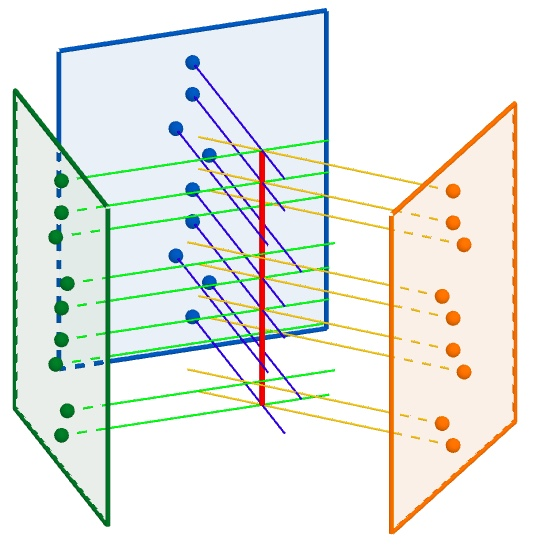
\includegraphics[scale=0.6]{131}

	Рис. 2.4: Построение скрещивающихся прямых через точки множеств.
\end{center}

\begin{center}
	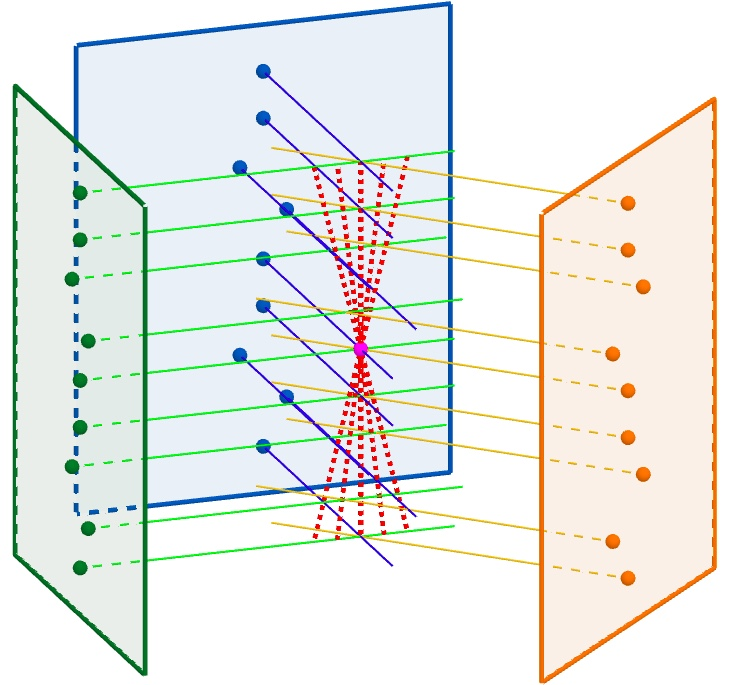
\includegraphics[scale=0.48]{132}

	Рис. 2.5: Изменение вектора прямой при фиксированной точке.

	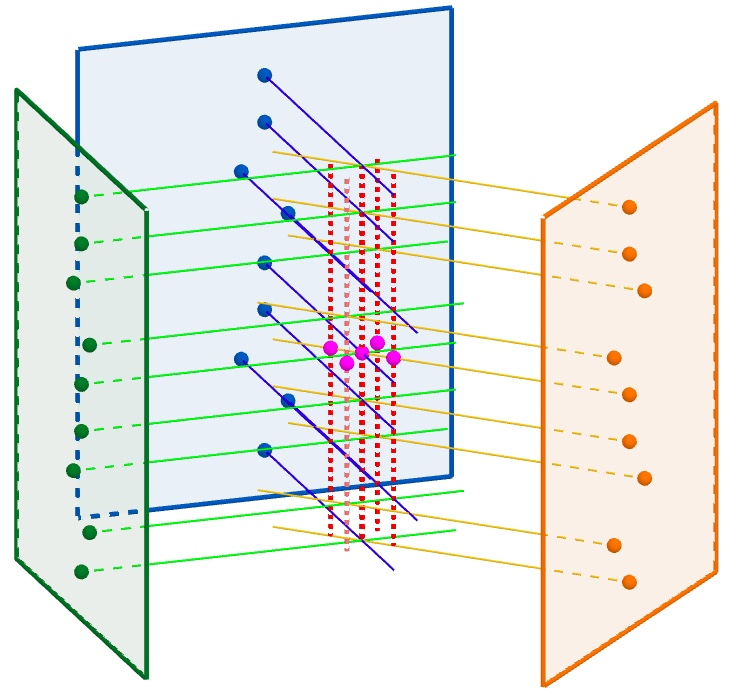
\includegraphics[scale=0.48]{133}

	Рис. 2.6: Изменение точки прямой при фиксированном векторе.
\end{center}

\subsection{Решение}\label{math3:solution}

Пусть имеем три множества:

\begin{center}
	$P_1 = \Set{p_i^1 = (x_i^1, y_i^1, z_i^1)}{i=\ton n_1}$

	\vspace{0.3cm}
	$P_2 = \Set{p_i^2 = (x_i^2, y_i^2, z_i^2)}{i=\ton n_2}$

	\vspace{0.3cm}
	$P_3 = \Set{p_i^3 = (x_i^3, y_i^3, z_i^3)}{i=\ton n_3}$
\end{center}

Также имеем три направления проектирования (векторы нормали плоскостей, которым принадлежат множества $P_1, P_2$ и $P_3$):
$$\begin{gathered}
	r_1 = (r_1^1, r_2^1, r_3^1) \\
	r_2 = (r_1^2, r_2^2, r_3^2) \\
	r_3 = (r_1^3, r_2^3, r_3^3)
\end{gathered}$$

Тогда имеем три набора прямых, причем внутри каждого набора прямые параллельны, а прямые разных наборов либо пересекаются, либо скрещиваются:

\begin{center}
	$S_1 = \Set{l_i^1:= \; \begin{cases}
		x = x_i^1 + r_1^1 \cdot t \\
		y = y_i^1 + r_2^1 \cdot t \\
		z = z_i^1 + r_3^1 \cdot t
	\end{cases}\text{, где }t \in \mathbb{R}\text{ - параметр}}{i=\ton n_1}$

	\vspace{0.3cm}
	$S_2 = \Set{l_i^2:= \; \begin{cases}
		x = x_i^2 + r_1^2 \cdot t \\
		y = y_i^2 + r_2^2 \cdot t \\
		z = z_i^2 + r_3^2 \cdot t
	\end{cases}\text{, где }t \in \mathbb{R}\text{ - параметр}}{i=\ton n_2}$

	\vspace{0.3cm}
	$S_3 = \Set{l_i^3:= \; \begin{cases}
		x = x_i^3 + r_1^3 \cdot t \\
		y = y_i^3 + r_2^3 \cdot t \\
		z = z_i^3 + r_3^3 \cdot t
	\end{cases}\text{, где }t \in \mathbb{R}\text{ - параметр}}{i=\ton n_3}$
\end{center}

\vspace{0.5cm}
Будем искать прямую в параметрическом виде. Пусть $(m, n, p)$ - напрявляющий вектор прямой, $(x_0, y_0, z_0)$ - некоторая точка прямой. Тогда следующая система задает прямую в $\mathbb{R}^3$: 

\begin{center}
	$\mathit{l}: \; \begin{cases}
		x = x_0 + m \cdot t \\
		y = y_0 + n \cdot t \\
		z = z_0 + p \cdot t
	\end{cases}$, где $t \in \mathbb{R}$ - параметр. 
\end{center}

\newpage
По определению расстояние от прямой $l_i^j$ до прямой $\mathit{l}$ определяется по следующей формуле:

$r_i^j = ((0,0,0), (x_i^j, y_i^j, z_i^j))$ - радиус-вектор точки на прямой $l_i^j$

$r_0 = ((0,0,0), (x_0, y_0, z_0))$ - радиус-вектор точки на прямой $\mathit{l}$

$\mathit{l} = (m, n, p)$ - напрявляющий вектор прямой $\mathit{l}$

$$d (l_i^j, \mathit{l}) = \frac{|(r_0 - r_i^j, \mathit{l}, r_j)|}{|[\mathit{l}, r_j]|}$$

Распишем составляющие элементы формулы для расстояния:

$$\begin{gathered}
	\text{[}l, r_j \text{]}= 
		\begin{vmatrix}
			\mathbf{i} & \mathbf{j} & \mathbf{k} \\
			m & n & p \\
			r_1^j & r_2^j & r_3^j
		\end{vmatrix} 
		= 
		\left(
			\begin{vmatrix}
				n & p \\
				r_2^j & r_3^j
			\end{vmatrix}, 
			-\begin{vmatrix}
				m & p \\
				r_1^j & r_3^j
			\end{vmatrix},
			\begin{vmatrix}
				m & n \\
				r_1^j & r_2^j
			\end{vmatrix}
		\right) = \\
		= (n r_3^j - p r_2^j, p r_1^j - m r_3^j, m r_2^j - n r_1^j)
\end{gathered}$$
$$|\text{[}l, r_j \text{]}| = \sqrt{ (n r_3^j - p r_2^j)^2 + (p r_1^j - m r_3^j)^2 + (m r_2^j - n r_1^j)^2}$$

$$\begin{gathered}
	|(r_0 - r_i^j, \mathit{l}, r_j)| = 
	\left| \begin{vmatrix}
		x_0 - x_i^j & y_0 - y_i^j & z_0 - z_i^j \\
		m & n & p \\
		r_1^j & r_2^j & r_3^j 
	\end{vmatrix} \right|= \\
	= \left| (x_0 - x_i^j) \begin{vmatrix}
		n & p \\
		r_2^j & r_3^j 
	\end{vmatrix} - (y_0 - y_i^j) \begin{vmatrix}
		m & p \\
		r_1^j & r_3^j
	\end{vmatrix} + (z_0 - z_i^j) \begin{vmatrix}
		m & n \\
		r_1^j & r_2^j
	\end{vmatrix} \right| = \\
	= \left| (x_0 - x_i^j)(n r_3^j - p r_2^j) - (y_0 - y_i^j)(m r_3^j - p r_1^j) + (z_0 - z_i^j)(m r_2^j - n r_1^j) \right| = \\
	= \left| \triangle_{ij}^x (n r_3^j - p r_2^j) - \triangle_{ij}^y (m r_3^j - p r_1^j) + \triangle_{ij}^z (m r_2^j - n r_1^j) \right|, \text{ где } \begin{cases}
		\triangle_{ij}^x = x_0 - x_i^j \\
		\triangle_{ij}^y = y_0 - y_i^j \\
		\triangle_{ij}^z = z_0 - z_i^j \\
	\end{cases}
\end{gathered}$$

Тогда формула расстояния принимает вид:
$$d (l_i^j, \mathit{l}) = \left| \frac{\triangle_{ij}^x (n r_3^j - p r_2^j) - \triangle_{ij}^y (m r_3^j - p r_1^j) + \triangle_{ij}^z (m r_2^j - n r_1^j)}{\sqrt{ (n r_3^j - p r_2^j)^2 + (p r_1^j - m r_3^j)^2 + (m r_2^j - n r_1^j)^2}} \right|$$

Тогда наша мера примет вид:

$$\begin{gathered}
	\Lambda = \sqrt{ 
	\underset{j=1}{\overset{3}{\sum}} 
	\underset{i=1}{\overset{n_1, n_2, n_3}{\sum}}
		\frac{\left(\triangle_{ij}^x (n r_3^j - p r_2^j) - \triangle_{ij}^y (m r_3^j - p r_1^j) + \triangle_{ij}^z (m r_2^j - n r_1^j)\right)^2}{(n r_3^j - p r_2^j)^2 + (p r_1^j - m r_3^j)^2 + (m r_2^j - n r_1^j)^2}
	 } 
\end{gathered}$$

Будем исследовать не саму меру, а подкоренное выражение.

Таким образом, задача свелась к поиску минимального значения выражения
$$\underset{j=1}{\overset{3}{\sum}} \underset{i=1}{\overset{n_1, n_2, n_3}{\sum}}
\frac{\left(\triangle_{ij}^x (n r_3^j - p r_2^j) - \triangle_{ij}^y (m r_3^j - p r_1^j) + \triangle_{ij}^z (m r_2^j - n r_1^j)\right)^2}{(n r_3^j - p r_2^j)^2 + (p r_1^j - m r_3^j)^2 + (m r_2^j - n r_1^j)^2}$$
по шести параметрам: $m,n,p$ (компоненты вектора искомой прямой) и $x_0, y_0, z_0$ (координаты точки, лежащей на искомой прямой).\\

Распишем знаменатель выражения:
$$\begin{gathered}
	(n r_3^j - p r_2^j)^2 + (p r_1^j - m r_3^j)^2 + (m r_2^j - n r_1^j)^2 = \\
	= n^2 (r_3^j)^2 + p^2 (r_2^j)^2 - 2 n p r_2^j r_3^j + \\
	+ p^2 (r_1^j)^2 + m^2 (r_3^j)^2 - 2 m p r_1^j r_3^j + \\
	+ m^2 (r_2^j)^2 + n^2 (r_1^j)^2 - 2 m n r_1^j r_2^j = \\
	= m^2 \left((r_2^j)^2 + (r_3^j)^2\right) + n^2 \left((r_1^j)^2 + (r_3^j)^2\right) + p^2 \left((r_1^j)^2 + (r_2^j)^2\right) - \\
	- 2 (m n r_1^j r_2^j + m p r_1^j r_3^j + n p r_2^j r_3^j)
\end{gathered}$$

Распишем числитель выражения:
$$\begin{gathered}
	\left(\triangle_{ij}^x (n r_3^j - p r_2^j) - \triangle_{ij}^y (m r_3^j - p r_1^j) + \triangle_{ij}^z (m r_2^j - n r_1^j)\right)^2 = \\
	= \left(\triangle_{ij}^x (n r_3^j - p r_2^j) \right)^2 + \left( \triangle_{ij}^y (m r_3^j - p r_1^j) \right)^2 + \left( \triangle_{ij}^z (m r_2^j - n r_1^j) \right)^2 - \\
	- 2 \left(\triangle_{ij}^x (n r_3^j - p r_2^j) \right)\left( \triangle_{ij}^y (m r_3^j - p r_1^j) \right) + \\
	+ 2 \left(\triangle_{ij}^x (n r_3^j - p r_2^j) \right) \left( \triangle_{ij}^z (m r_2^j - n r_1^j) \right) - \\
	- 2\left( \triangle_{ij}^y (m r_3^j - p r_1^j) \right)\left( \triangle_{ij}^z (m r_2^j - n r_1^j) \right) =
\end{gathered}$$

$$\begin{gathered}
	= \left(\triangle_{ij}^x\right)^2 (n r_3^j - p r_2^j)^2  + \left( \triangle_{ij}^y\right)^2 (m r_3^j - p r_1^j)^2  + \left( \triangle_{ij}^z \right)^2 (m r_2^j - n r_1^j)^2 - \\
	- 2 \triangle_{ij}^x \triangle_{ij}^y (n r_3^j - p r_2^j) (m r_3^j - p r_1^j) + \\
	+ 2 \triangle_{ij}^x  \triangle_{ij}^z (n r_3^j - p r_2^j)  (m r_2^j - n r_1^j) - \\
	- 2 \triangle_{ij}^y  \triangle_{ij}^z (m r_3^j - p r_1^j)  (m r_2^j - n r_1^j) =
\end{gathered}$$
\newpage
$$\begin{gathered}
	= \left(\triangle_{ij}^x\right)^2 (n^2 (r_3^j)^2 + p^2 (r_2^j)^2 - 2 n p r_2^j r_3^j)  + \\
	+  \left( \triangle_{ij}^y\right)^2 (m^2 (r_3^j)^2 + p^2 (r_1^j)^2 - 2 m p r_1^j r_3^j)  + \\
	+ \left( \triangle_{ij}^z \right)^2 (m^2 (r_2^j)^2 + n^2 (r_1^j)^2 - 2 m n r_1^j r_2^j) - \\
	- 2 \triangle_{ij}^x \triangle_{ij}^y (m n (r_3^j)^2 + p^2 r_1^j r_2^j - m p r_2^j r_3^j - n p r_1^j r_3^j) + \\
	+ 2 \triangle_{ij}^x  \triangle_{ij}^z (m n r_2^j r_3^j + n p r_1^j r_2^j - m p (r_2^j)^2 - n^2 r_1^j r_3^j) - \\
	- 2 \triangle_{ij}^y  \triangle_{ij}^z (m^2 r_2^j r_3^j + n p (r_1^j)^2 - m n r_1^j r_3^j - m p r_1^j r_2^j) = 
\end{gathered}$$

$$\begin{gathered}
	= m^2 \left( \left( \triangle_{ij}^y\right)^2 (r_3^j)^2 + \left( \triangle_{ij}^z \right)^2 (r_2^j)^2 - 2 \triangle_{ij}^y  \triangle_{ij}^z r_2^j r_3^j \right) + \\
	+ n^2 \left( \left(\triangle_{ij}^x\right)^2 (r_3^j)^2 + \left( \triangle_{ij}^z \right)^2 (r_1^j)^2 - 2 \triangle_{ij}^x  \triangle_{ij}^z r_1^j r_3^j \right) + \\
	+ p^2 \left( \left(\triangle_{ij}^x\right)^2 (r_2^j)^2 + \left( \triangle_{ij}^y\right)^2 (r_1^j)^2 - 2 \triangle_{ij}^x \triangle_{ij}^y r_1^j r_2^j \right) + \\
	+ m n \left( - 2 \left( \triangle_{ij}^z \right)^2 r_1^j r_2^j - 2 \triangle_{ij}^x \triangle_{ij}^y (r_3^j)^2 + 2 \triangle_{ij}^x  \triangle_{ij}^z r_2^j r_3^j + 2 \triangle_{ij}^y  \triangle_{ij}^z r_1^j r_3^j \right) + \\
	+ m p \left( -2 \left( \triangle_{ij}^y\right)^2 r_1^j r_3^j + 2 \triangle_{ij}^x \triangle_{ij}^y r_2^j r_3^j - 2 \triangle_{ij}^x  \triangle_{ij}^z (r_2^j)^2 + 2 \triangle_{ij}^y  \triangle_{ij}^z r_1^j r_2^j \right) + \\
	+ n p \left( -2 \left(\triangle_{ij}^x\right)^2 r_2^j r_3^j + 2 \triangle_{ij}^x \triangle_{ij}^y r_1^j r_3^j + 2 \triangle_{ij}^x  \triangle_{ij}^z r_1^j r_2^j - 2 \triangle_{ij}^y  \triangle_{ij}^z (r_1^j)^2 \right) =
\end{gathered}$$

$$\begin{gathered}
	= m^2 \left( \triangle_{ij}^y r_3^j - \triangle_{ij}^z r_2^j \right)^2 
	+ n^2 \left( \triangle_{ij}^x r_3^j - \triangle_{ij}^z r_1^j \right)^2
	+ p^2 \left( \triangle_{ij}^x r_2^j - \triangle_{ij}^y r_1^j \right)^2 + \\
	+ 2 m n \left( - \left( \triangle_{ij}^z \right)^2 r_1^j r_2^j - \triangle_{ij}^x \triangle_{ij}^y (r_3^j)^2 + \triangle_{ij}^x  \triangle_{ij}^z r_2^j r_3^j + \triangle_{ij}^y  \triangle_{ij}^z r_1^j r_3^j \right) + \\
	+ 2 m p \left( - \left( \triangle_{ij}^y\right)^2 r_1^j r_3^j +  \triangle_{ij}^x \triangle_{ij}^y r_2^j r_3^j -  \triangle_{ij}^x  \triangle_{ij}^z (r_2^j)^2 +  \triangle_{ij}^y  \triangle_{ij}^z r_1^j r_2^j \right) + \\
	+ 2 n p \left( - \left(\triangle_{ij}^x\right)^2 r_2^j r_3^j +  \triangle_{ij}^x \triangle_{ij}^y r_1^j r_3^j +  \triangle_{ij}^x  \triangle_{ij}^z r_1^j r_2^j -  \triangle_{ij}^y  \triangle_{ij}^z (r_1^j)^2 \right)
\end{gathered}$$

Рассмотрим наше выражение как функцию от трех переменных $x_0, y_0, z_0$ при фиксированных $m, n, p$. Найдем частные производные выражения по переменным $x_0, y_0, z_0$. Заметим, что от этих переменных зависят только части $\triangle_{ij}^x, \triangle_{ij}^y, \triangle_{ij}^z$, а знаменатель от них не зависит, значит при нахождении минимального значения знаменатель можно не учитывать. Частные производные числителя:
$$\begin{cases}
	\frac{\partial}{\partial x_0} \underset{j=1}{\overset{3}{\sum}} \underset{i=1}{\overset{n_1, n_2, n_3}{\sum}} \left(\triangle_{ij}^x (n r_3^j - p r_2^j) - \triangle_{ij}^y (m r_3^j - p r_1^j) + \triangle_{ij}^z (m r_2^j - n r_1^j)\right)^2 = 0 \\
	\frac{\partial}{\partial y_0} \underset{j=1}{\overset{3}{\sum}} \underset{i=1}{\overset{n_1, n_2, n_3}{\sum}} \left(\triangle_{ij}^x (n r_3^j - p r_2^j) - \triangle_{ij}^y (m r_3^j - p r_1^j) + \triangle_{ij}^z (m r_2^j - n r_1^j)\right)^2 = 0 \\
	\frac{\partial}{\partial z_0} \underset{j=1}{\overset{3}{\sum}} \underset{i=1}{\overset{n_1, n_2, n_3}{\sum}} \left(\triangle_{ij}^x (n r_3^j - p r_2^j) - \triangle_{ij}^y (m r_3^j - p r_1^j) + \triangle_{ij}^z (m r_2^j - n r_1^j)\right)^2 = 0
\end{cases} \; \Leftrightarrow $$
\hfill \break \hfill \break \hfill \break
$$ \Leftrightarrow \; \begin{cases}
	\underset{j=1}{\overset{3}{\sum}} \underset{i=1}{\overset{n_1, n_2, n_3}{\sum}} \Bigg( 2 \triangle_{ij}^x (n^2 (r_3^j)^2 + p^2 (r_2^j)^2 - 2 n p r_2^j r_3^j) - \\
	\hspace{1cm} - 2 \triangle_{ij}^y (m n (r_3^j)^2 + p^2 r_1^j r_2^j - m p r_2^j r_3^j - n p r_1^j r_3^j) + \\
	\hspace{2cm} + 2 \triangle_{ij}^z (m n r_2^j r_3^j + n p r_1^j r_2^j - m p (r_2^j)^2 - n^2 r_1^j r_3^j) \Bigg)= 0 \\
	\underset{j=1}{\overset{3}{\sum}} \underset{i=1}{\overset{n_1, n_2, n_3}{\sum}} \Bigg( 2 \triangle_{ij}^y (m^2 (r_3^j)^2 + p^2 (r_1^j)^2 - 2 m p r_1^j r_3^j) - \\
	\hspace{1cm} - 2 \triangle_{ij}^x (m n (r_3^j)^2 + p^2 r_1^j r_2^j - m p r_2^j r_3^j - n p r_1^j r_3^j) - \\
	\hspace{2cm} - 2 \triangle_{ij}^z (m^2 r_2^j r_3^j + n p (r_1^j)^2 - m n r_1^j r_3^j - m p r_1^j r_2^j) \Bigg) = 0 \\
	\underset{j=1}{\overset{3}{\sum}} \underset{i=1}{\overset{n_1, n_2, n_3}{\sum}} \Bigg( 2 \triangle_{ij}^z (m^2 (r_2^j)^2 + n^2 (r_1^j)^2 - 2 m n r_1^j r_2^j) + \\
	\hspace{1cm} + 2 \triangle_{ij}^x (m n r_2^j r_3^j + n p r_1^j r_2^j - m p (r_2^j)^2 - n^2 r_1^j r_3^j) - \\
	\hspace{2cm} - 2 \triangle_{ij}^y (m^2 r_2^j r_3^j + n p (r_1^j)^2 - m n r_1^j r_3^j - m p r_1^j r_2^j) \Bigg) = 0
\end{cases} \; \Leftrightarrow$$
$$ \Leftrightarrow \; \begin{cases}
	\underset{j=1}{\overset{3}{\sum}} \underset{i=1}{\overset{n_1, n_2, n_3}{\sum}} \Bigg( \triangle_{ij}^x (n r_3^j - p r_2^j)^2 - \triangle_{ij}^y (m r_3^j - p r_1^j) (n r_3^j - p r_2^j) + \\
	\hspace{1.5cm} + \triangle_{ij}^z (m r_2^j - n r_1^j) (n r_3^j - p r_2^j) \Bigg) = 0 \\
	\underset{j=1}{\overset{3}{\sum}} \underset{i=1}{\overset{n_1, n_2, n_3}{\sum}} \Bigg( \triangle_{ij}^y (m r_3^j - p r_1^j)^2 - \triangle_{ij}^x (m r_3^j - p r_1^j) (n r_3^j - p r_2^j) - \\
	\hspace{1.5cm} - \triangle_{ij}^z (m r_2^j - n r_1^j) (m r_3^j - p r_1^j) \Bigg) = 0 \\
	\underset{j=1}{\overset{3}{\sum}} \underset{i=1}{\overset{n_1, n_2, n_3}{\sum}} \Bigg( \triangle_{ij}^z (m r_2^j - n r_1^j)^2 + \triangle_{ij}^x (m r_2^j - n r_1^j) (n r_3^j - p r_2^j) - \\
	\hspace{1.5cm} - \triangle_{ij}^y (m r_2^j - n r_1^j) (m r_3^j - p r_1^j) \Bigg) = 0
\end{cases} \; \Leftrightarrow$$
\hfill \break \hfill \break \hfill \break \hfill \break \hfill \break
\hfill \break \hfill \break \hfill \break
$$ \Leftrightarrow \; \begin{cases}
	\underset{i=1}{\overset{n_1, n_2, n_3}{\sum}} \Bigg( 
		\triangle_{i1}^x (n r_3^1 - p r_2^1)^2 - \triangle_{i1}^y (m r_3^1 - p r_1^1) (n r_3^1 - p r_2^1) + \\
		\hspace{1.5cm} + \triangle_{i1}^z (m r_2^1 - n r_1^1) (n r_3^1 - p r_2^1) + \\
		\hspace{1.5cm} + \triangle_{i2}^x (n r_3^2 - p r_2^2)^2 - \triangle_{i2}^y (m r_3^2 - p r_1^2) (n r_3^2 - p r_2^2) + \\
		\hspace{1.5cm} + \triangle_{i2}^z (m r_2^2 - n r_1^2) (n r_3^2 - p r_2^2) + \\
		\hspace{1.5cm} + \triangle_{i3}^x (n r_3^3 - p r_2^3)^2 - \triangle_{i3}^y (m r_3^3 - p r_1^3) (n r_3^3 - p r_2^3) + \\
		\hspace{1.5cm} + \triangle_{i3}^z (m r_2^3 - n r_1^3) (n r_3^3 - p r_2^3) \Bigg) = 0 \\
	\underset{i=1}{\overset{n_1, n_2, n_3}{\sum}} \Bigg( 
		\triangle_{i1}^y (m r_3^1 - p r_1^1)^2 - \triangle_{i1}^x (m r_3^1 - p r_1^1) (n r_3^1 - p r_2^1) - \\
		\hspace{1.5cm} - \triangle_{i1}^z (m r_2^1 - n r_1^1) (m r_3^1 - p r_1^1) + \\
		\hspace{1.5cm} + \triangle_{i2}^y (m r_3^2 - p r_1^2)^2 - \triangle_{i2}^x (m r_3^2 - p r_1^2) (n r_3^2 - p r_2^2) - \\
		\hspace{1.5cm} - \triangle_{i2}^z (m r_2^2 - n r_1^2) (m r_3^2 - p r_1^2) + \\
		\hspace{1.5cm} + \triangle_{i3}^y (m r_3^3 - p r_1^3)^2 - \triangle_{i3}^x (m r_3^3 - p r_1^3) (n r_3^3 - p r_2^3) - \\
		\hspace{1.5cm} - \triangle_{i3}^z (m r_2^3 - n r_1^3) (m r_3^3 - p r_1^3) \Bigg) = 0 \\
	\underset{i=1}{\overset{n_1, n_2, n_3}{\sum}} \Bigg( 
		\triangle_{i1}^z (m r_2^1 - n r_1^1)^2 + \triangle_{i1}^x (m r_2^1 - n r_1^1) (n r_3^1 - p r_2^1) - \\
		\hspace{1.5cm} - \triangle_{i1}^y (m r_2^1 - n r_1^1) (m r_3^1 - p r_1^1) + \\
		\hspace{1.5cm} + \triangle_{i2}^z (m r_2^2 - n r_1^2)^2 + \triangle_{i2}^x (m r_2^2 - n r_1^2) (n r_3^2 - p r_2^2) - \\
		\hspace{1.5cm} - \triangle_{i2}^y (m r_2^2 - n r_1^2) (m r_3^2 - p r_1^2) + \\
		\hspace{1.5cm} + \triangle_{i3}^z (m r_2^3 - n r_1^3)^2 + \triangle_{i3}^x (m r_2^3 - n r_1^3) (n r_3^3 - p r_2^3) - \\
		\hspace{1.5cm} - \triangle_{i3}^y (m r_2^3 - n r_1^3) (m r_3^3 - p r_1^3) \Bigg) = 0
\end{cases} \; \Leftrightarrow$$
\hfill \break \hfill \break
$$ \Leftrightarrow \; \begin{cases}
	\underset{i=1}{\overset{n_1, n_2, n_3}{\sum}} \Bigg( 
		(x_0 - x_i^1) (n r_3^1 - p r_2^1)^2 - \\
		\hspace{1.5cm} - (y_0 - y_i^1) (m r_3^1 - p r_1^1) (n r_3^1 - p r_2^1) + \\
		\hspace{1.5cm} + (z_0 - z_i^1) (m r_2^1 - n r_1^1) (n r_3^1 - p r_2^1) + \\
		\hspace{1.5cm} + (x_0 - x_i^2) (n r_3^2 - p r_2^2)^2 - \\
		\hspace{1.5cm} - (y_0 - y_i^2) (m r_3^2 - p r_1^2) (n r_3^2 - p r_2^2) + \\
		\hspace{1.5cm} + (z_0 - z_i^2) (m r_2^2 - n r_1^2) (n r_3^2 - p r_2^2) + \\
		\hspace{1.5cm} + (x_0 - x_i^3) (n r_3^3 - p r_2^3)^2 - \\
		\hspace{1.5cm} - (y_0 - y_i^3) (m r_3^3 - p r_1^3) (n r_3^3 - p r_2^3) + \\
		\hspace{1.5cm} + (z_0 - z_i^3) (m r_2^3 - n r_1^3) (n r_3^3 - p r_2^3) \Bigg) = 0 \\
	\underset{i=1}{\overset{n_1, n_2, n_3}{\sum}} \Bigg( 
		(y_0 - y_i^1) (m r_3^1 - p r_1^1)^2 - \\
		\hspace{1.5cm} - (x_0 - x_i^1) (m r_3^1 - p r_1^1) (n r_3^1 - p r_2^1) - \\
		\hspace{1.5cm} - (z_0 - z_i^1) (m r_2^1 - n r_1^1) (m r_3^1 - p r_1^1) + \\
		\hspace{1.5cm} + (y_0 - y_i^2) (m r_3^2 - p r_1^2)^2 - \\
		\hspace{1.5cm} - (x_0 - x_i^2) (m r_3^2 - p r_1^2) (n r_3^2 - p r_2^2) - \\
		\hspace{1.5cm} - (z_0 - z_i^2) (m r_2^2 - n r_1^2) (m r_3^2 - p r_1^2) + \\
		\hspace{1.5cm} + (y_0 - y_i^3) (m r_3^3 - p r_1^3)^2 - \\
		\hspace{1.5cm} - (x_0 - x_i^3) (m r_3^3 - p r_1^3) (n r_3^3 - p r_2^3) - \\
		\hspace{1.5cm} - (z_0 - z_i^3) (m r_2^3 - n r_1^3) (m r_3^3 - p r_1^3) \Bigg) = 0 \\
	\underset{i=1}{\overset{n_1, n_2, n_3}{\sum}} \Bigg( 
		(z_0 - z_i^1) (m r_2^1 - n r_1^1)^2 + \\
		\hspace{1.5cm} + (x_0 - x_i^1) (m r_2^1 - n r_1^1) (n r_3^1 - p r_2^1) - \\
		\hspace{1.5cm} - (y_0 - y_i^1) (m r_2^1 - n r_1^1) (m r_3^1 - p r_1^1) + \\
		\hspace{1.5cm} + (z_0 - z_i^2) (m r_2^2 - n r_1^2)^2 + \\
		\hspace{1.5cm} + (x_0 - x_i^2) (m r_2^2 - n r_1^2) (n r_3^2 - p r_2^2) - \\
		\hspace{1.5cm} - (y_0 - y_i^2) (m r_2^2 - n r_1^2) (m r_3^2 - p r_1^2) + \\
		\hspace{1.5cm} + (z_0 - z_i^3) (m r_2^3 - n r_1^3)^2 + \\
		\hspace{1.5cm} + (x_0 - x_i^3) (m r_2^3 - n r_1^3) (n r_3^3 - p r_2^3) - \\
		\hspace{1.5cm} - (y_0 - y_i^3) (m r_2^3 - n r_1^3) (m r_3^3 - p r_1^3) \Bigg) = 0
\end{cases} \; \Leftrightarrow$$

Первое уравнение системы:
$$\begin{gathered}
	(n_1 + n_2 + n_3) x_0 (n r_3^1 - p r_2^1)^2 - \underset{i=1}{\overset{n_1, n_2, n_3}{\sum}} x_i^1 (n r_3^1 - p r_2^1)^2 - \\
	\hspace{0.5cm} - (n_1 + n_2 + n_3)y_0 (m r_3^1 - p r_1^1) (n r_3^1 - p r_2^1) + \underset{i=1}{\overset{n_1, n_2, n_3}{\sum}} y_i^1 (m r_3^1 - p r_1^1) (n r_3^1 - p r_2^1) + \\
	\hspace{0.5cm} + (n_1 + n_2 + n_3) z_0 (m r_2^1 - n r_1^1) (n r_3^1 - p r_2^1) - \underset{i=1}{\overset{n_1, n_2, n_3}{\sum}} z_i^1  (m r_2^1 - n r_1^1) (n r_3^1 - p r_2^1) + \\
	\hspace{0.5cm} + (n_1 + n_2 + n_3) x_0 (n r_3^2 - p r_2^2)^2 - \underset{i=1}{\overset{n_1, n_2, n_3}{\sum}} x_i^2 (n r_3^2 - p r_2^2)^2 - \\
	\hspace{0.5cm} - (n_1 + n_2 + n_3) y_0 (m r_3^2 - p r_1^2) (n r_3^2 - p r_2^2) + \underset{i=1}{\overset{n_1, n_2, n_3}{\sum}} y_i^2  (m r_3^2 - p r_1^2) (n r_3^2 - p r_2^2) + \\
	\hspace{0.5cm} + (n_1 + n_2 + n_3) z_0 (m r_2^2 - n r_1^2) (n r_3^2 - p r_2^2) - \underset{i=1}{\overset{n_1, n_2, n_3}{\sum}} z_i^2 (m r_2^2 - n r_1^2) (n r_3^2 - p r_2^2) + \\
	\hspace{0.5cm} + (n_1 + n_2 + n_3) x_0 (n r_3^3 - p r_2^3)^2 - \underset{i=1}{\overset{n_1, n_2, n_3}{\sum}} x_i^3 (n r_3^3 - p r_2^3)^2 - \\
	\hspace{0.5cm} - (n_1 + n_2 + n_3) y_0 (m r_3^3 - p r_1^3) (n r_3^3 - p r_2^3) + \underset{i=1}{\overset{n_1, n_2, n_3}{\sum}} y_i^3 (m r_3^3 - p r_1^3) (n r_3^3 - p r_2^3) + \\
	\hspace{0.5cm} + (n_1 + n_2 + n_3) z_0 (m r_2^3 - n r_1^3) (n r_3^3 - p r_2^3) - \underset{i=1}{\overset{n_1, n_2, n_3}{\sum}} z_i^3 (m r_2^3 - n r_1^3) (n r_3^3 - p r_2^3) = 0
\end{gathered}$$
Сгруппируем члены, получим приведенный вид первого уравнения:
$$\begin{gathered}
	x_0 \bigg( (n r_3^1 - p r_2^1)^2 + (n r_3^2 - p r_2^2)^2 + (n r_3^3 - p r_2^3)^2 \bigg) + \\
	+ y_0 \bigg( -(m r_3^1 - p r_1^1) (n r_3^1 - p r_2^1) - (m r_3^2 - p r_1^2) (n r_3^2 - p r_2^2) - (m r_3^3 - p r_1^3) (n r_3^3 - p r_2^3) \bigg) + \\
	+ z_0 \bigg( (m r_2^1 - n r_1^1) (n r_3^1 - p r_2^1) + (m r_2^2 - n r_1^2) (n r_3^2 - p r_2^2) + (m r_2^3 - n r_1^3) (n r_3^3 - p r_2^3) \bigg) + \\
	+ \frac{1}{n_1+n_2+n_3} \underset{i=1}{\overset{n_1, n_2, n_3}{\sum}} \bigg( 
		- x_i^1 (n r_3^1 - p r_2^1)^2 +
		y_i^1 (m r_3^1 - p r_1^1) (n r_3^1 - p r_2^1) - \\
		- z_i^1  (m r_2^1 - n r_1^1) (n r_3^1 - p r_2^1) - 
		x_i^2 (n r_3^2 - p r_2^2)^2 + \\
		+ y_i^2  (m r_3^2 - p r_1^2) (n r_3^2 - p r_2^2) -
		z_i^2 (m r_2^2 - n r_1^2) (n r_3^2 - p r_2^2) - \\
		- x_i^3 (n r_3^3 - p r_2^3)^2 +
		y_i^3 (m r_3^3 - p r_1^3) (n r_3^3 - p r_2^3) -
		z_i^3 (m r_2^3 - n r_1^3) (n r_3^3 - p r_2^3)
	 \bigg) = 0
\end{gathered}$$

Второе уравнение системы:
$$\begin{gathered}
	(n_1 + n_2 + n_3) y_0 (m r_3^1 - p r_1^1)^2 - \underset{i=1}{\overset{n_1, n_2, n_3}{\sum}} y_i^1 (m r_3^1 - p r_1^1)^2 - \\
	\hspace{0.5cm} - (n_1 + n_2 + n_3) x_0 (m r_3^1 - p r_1^1) (n r_3^1 - p r_2^1) + \underset{i=1}{\overset{n_1, n_2, n_3}{\sum}} x_i^1 (m r_3^1 - p r_1^1) (n r_3^1 - p r_2^1) + \\
	\hspace{0.5cm} + (n_1 + n_2 + n_3) z_0 (m r_2^1 - n r_1^1) (m r_3^1 - p r_1^1) - \underset{i=1}{\overset{n_1, n_2, n_3}{\sum}} z_i^1  (m r_2^1 - n r_1^1) (m r_3^1 - p r_1^1) + \\
	\hspace{0.5cm} + (n_1 + n_2 + n_3) y_0 (m r_3^2 - p r_1^2)^2 - \underset{i=1}{\overset{n_1, n_2, n_3}{\sum}} y_i^2 (m r_3^2 - p r_1^2)^2 - \\
	\hspace{0.5cm} - (n_1 + n_2 + n_3) x_0 (m r_3^2 - p r_1^2) (n r_3^2 - p r_2^2) + \underset{i=1}{\overset{n_1, n_2, n_3}{\sum}} x_i^2  (m r_3^2 - p r_1^2) (n r_3^2 - p r_2^2) + \\
	\hspace{0.5cm} + (n_1 + n_2 + n_3) z_0 (m r_2^2 - n r_1^2) (m r_3^2 - p r_1^2) - \underset{i=1}{\overset{n_1, n_2, n_3}{\sum}} z_i^2 (m r_2^2 - n r_1^2) (m r_3^2 - p r_1^2) + \\
	\hspace{0.5cm} + (n_1 + n_2 + n_3) y_0 (m r_3^3 - p r_1^3)^2 - \underset{i=1}{\overset{n_1, n_2, n_3}{\sum}} y_i^3 (m r_3^3 - p r_1^3)^2 - \\
	\hspace{0.5cm} - (n_1 + n_2 + n_3) x_0 (m r_3^3 - p r_1^3) (n r_3^3 - p r_2^3) + \underset{i=1}{\overset{n_1, n_2, n_3}{\sum}} x_i^3 (m r_3^3 - p r_1^3) (n r_3^3 - p r_2^3) + \\
	\hspace{0.5cm} + (n_1 + n_2 + n_3) z_0 (m r_2^3 - n r_1^3) (m r_3^3 - p r_1^3) - \underset{i=1}{\overset{n_1, n_2, n_3}{\sum}} z_i^3 (m r_2^3 - n r_1^3) (m r_3^3 - p r_1^3) = 0
\end{gathered}$$
Сгруппируем члены, получим приведенный вид второго уравнения:
$$\begin{gathered}
	x_0 \bigg( -(m r_3^1 - p r_1^1) (n r_3^1 - p r_2^1) - (m r_3^2 - p r_1^2) (n r_3^2 - p r_2^2) - (m r_3^3 - p r_1^3) (n r_3^3 - p r_2^3) \bigg) + \\
	+ y_0 \bigg( (m r_3^1 - p r_1^1)^2 + (m r_3^2 - p r_1^2)^2 + (m r_3^3 - p r_1^3)^2 \bigg) + \\
	+ z_0 \bigg( (m r_2^1 - n r_1^1) (m r_3^1 - p r_1^1) + (m r_2^2 - n r_1^2) (m r_3^2 - p r_1^2) + (m r_2^3 - n r_1^3) (m r_3^3 - p r_1^3) \bigg) + \\
	+ \frac{1}{n_1+n_2+n_3} \underset{i=1}{\overset{n_1, n_2, n_3}{\sum}} \bigg( 
		- y_i^1 (m r_3^1 - p r_1^1)^2
		+ x_i^1 (m r_3^1 - p r_1^1) (n r_3^1 - p r_2^1) - \\
		- z_i^1  (m r_2^1 - n r_1^1) (m r_3^1 - p r_1^1)
		- y_i^2 (m r_3^2 - p r_1^2)^2 + \\
		+ x_i^2  (m r_3^2 - p r_1^2) (n r_3^2 - p r_2^2)
		- z_i^2 (m r_2^2 - n r_1^2) (m r_3^2 - p r_1^2) - \\
		- y_i^3 (m r_3^3 - p r_1^3)^2
		+ x_i^3 (m r_3^3 - p r_1^3) (n r_3^3 - p r_2^3)
		- z_i^3 (m r_2^3 - n r_1^3) (m r_3^3 - p r_1^3)
	 \bigg) = 0
\end{gathered}$$
Третье уравнение системы:
$$\begin{gathered}
	(n_1 + n_2 + n_3) z_0 (m r_2^1 - n r_1^1)^2 - \underset{i=1}{\overset{n_1, n_2, n_3}{\sum}} z_i^1 (m r_2^1 - n r_1^1)^2 - \\
	\hspace{0.5cm} - (n_1 + n_2 + n_3) x_0 (m r_2^1 - n r_1^1) (n r_3^1 - p r_2^1) + \underset{i=1}{\overset{n_1, n_2, n_3}{\sum}} x_i^1 (m r_2^1 - n r_1^1) (n r_3^1 - p r_2^1) + \\
	\hspace{0.5cm} + (n_1 + n_2 + n_3) y_0 (m r_2^1 - n r_1^1) (m r_3^1 - p r_1^1) - \underset{i=1}{\overset{n_1, n_2, n_3}{\sum}} y_i^1  (m r_2^1 - n r_1^1) (m r_3^1 - p r_1^1) + \\
	\hspace{0.5cm} + (n_1 + n_2 + n_3) z_0 (m r_2^2 - n r_1^2)^2 - \underset{i=1}{\overset{n_1, n_2, n_3}{\sum}} z_i^2 (m r_2^2 - n r_1^2)^2 - \\
	\hspace{0.5cm} - (n_1 + n_2 + n_3) x_0 (m r_2^2 - n r_1^2) (n r_3^2 - p r_2^2) + \underset{i=1}{\overset{n_1, n_2, n_3}{\sum}} x_i^2  (m r_2^2 - n r_1^2) (n r_3^2 - p r_2^2) + \\
	\hspace{0.5cm} + (n_1 + n_2 + n_3) y_0 (m r_2^2 - n r_1^2) (m r_3^2 - p r_1^2) - \underset{i=1}{\overset{n_1, n_2, n_3}{\sum}} y_i^2 (m r_2^2 - n r_1^2) (m r_3^2 - p r_1^2) + \\
	\hspace{0.5cm} + (n_1 + n_2 + n_3) z_0 (m r_2^3 - n r_1^3)^2 - \underset{i=1}{\overset{n_1, n_2, n_3}{\sum}} z_i^3 (m r_2^3 - n r_1^3)^2 - \\
	\hspace{0.5cm} - (n_1 + n_2 + n_3) x_0 (m r_2^3 - n r_1^3) (n r_3^3 - p r_2^3) + \underset{i=1}{\overset{n_1, n_2, n_3}{\sum}} x_i^3 (m r_2^3 - n r_1^3) (n r_3^3 - p r_2^3) + \\
	\hspace{0.5cm} + (n_1 + n_2 + n_3) y_0 (m r_2^3 - n r_1^3) (m r_3^3 - p r_1^3) - \underset{i=1}{\overset{n_1, n_2, n_3}{\sum}} y_i^3 (m r_2^3 - n r_1^3) (m r_3^3 - p r_1^3) = 0
\end{gathered}$$
Сгруппируем члены, получим приведенный вид третьего уравнения:
$$\begin{gathered}
	x_0 \bigg( - (m r_2^1 - n r_1^1) (n r_3^1 - p r_2^1) - (m r_2^2 - n r_1^2) (n r_3^2 - p r_2^2) - (m r_2^3 - n r_1^3) (n r_3^3 - p r_2^3) \bigg) + \\
	+ y_0 \bigg( (m r_2^1 - n r_1^1) (m r_3^1 - p r_1^1) + (m r_2^2 - n r_1^2) (m r_3^2 - p r_1^2) + (m r_2^3 - n r_1^3) (m r_3^3 - p r_1^3) \bigg) + \\
	+ z_0 \bigg( (m r_2^1 - n r_1^1)^2 + (m r_2^2 - n r_1^2)^2 + (m r_2^3 - n r_1^3)^2 \bigg) + \\
	+ \frac{1}{n_1+n_2+n_3} \underset{i=1}{\overset{n_1, n_2, n_3}{\sum}} \bigg( 
		- z_i^1 (m r_2^1 - n r_1^1)^2
		+ x_i^1 (m r_2^1 - n r_1^1) (n r_3^1 - p r_2^1) - \\
		- y_i^1  (m r_2^1 - n r_1^1) (m r_3^1 - p r_1^1)
		- z_i^2 (m r_2^2 - n r_1^2)^2 + \\
		+ x_i^2  (m r_2^2 - n r_1^2) (n r_3^2 - p r_2^2)
		- y_i^2 (m r_2^2 - n r_1^2) (m r_3^2 - p r_1^2)
		- z_i^3 (m r_2^3 - n r_1^3)^2\\
		+ x_i^3 (m r_2^3 - n r_1^3) (n r_3^3 - p r_2^3)
		- y_i^3 (m r_2^3 - n r_1^3) (m r_3^3 - p r_1^3)
	 \bigg) = 0
\end{gathered}$$

Введем обозначения:
$$\begin{cases}
	a_1 = (n r_3^1 - p r_2^1)^2 + (n r_3^2 - p r_2^2)^2 + (n r_3^3 - p r_2^3)^2 \\
	b_1 = -(m r_3^1 - p r_1^1) (n r_3^1 - p r_2^1) - (m r_3^2 - p r_1^2) (n r_3^2 - p r_2^2) - (m r_3^3 - p r_1^3) (n r_3^3 - p r_2^3) \\
	c_1 = (m r_2^1 - n r_1^1) (n r_3^1 - p r_2^1) + (m r_2^2 - n r_1^2) (n r_3^2 - p r_2^2) + (m r_2^3 - n r_1^3) (n r_3^3 - p r_2^3) \\
	d_1 = \frac{1}{n_1+n_2+n_3} \underset{i=1}{\overset{n_1, n_2, n_3}{\sum}} \bigg( 
		- x_i^1 (n r_3^1 - p r_2^1)^2 +
		y_i^1 (m r_3^1 - p r_1^1) (n r_3^1 - p r_2^1) - \\
		\hspace{1cm} - z_i^1  (m r_2^1 - n r_1^1) (n r_3^1 - p r_2^1) - 
		x_i^2 (n r_3^2 - p r_2^2)^2 + \\
		\hspace{1cm} + y_i^2  (m r_3^2 - p r_1^2) (n r_3^2 - p r_2^2) -
		z_i^2 (m r_2^2 - n r_1^2) (n r_3^2 - p r_2^2) - \\
		\hspace{1cm} - x_i^3 (n r_3^3 - p r_2^3)^2 +
		y_i^3 (m r_3^3 - p r_1^3) (n r_3^3 - p r_2^3) -
		z_i^3 (m r_2^3 - n r_1^3) (n r_3^3 - p r_2^3)
	 \bigg) \\
	a_2 = -(m r_3^1 - p r_1^1) (n r_3^1 - p r_2^1) - (m r_3^2 - p r_1^2) (n r_3^2 - p r_2^2) - (m r_3^3 - p r_1^3) (n r_3^3 - p r_2^3) \\
	b_2 = (m r_3^1 - p r_1^1)^2 + (m r_3^2 - p r_1^2)^2 + (m r_3^3 - p r_1^3)^2 \\
	c_2 = (m r_2^1 - n r_1^1) (m r_3^1 - p r_1^1) + (m r_2^2 - n r_1^2) (m r_3^2 - p r_1^2) + (m r_2^3 - n r_1^3) (m r_3^3 - p r_1^3) \\
	d_2 = \frac{1}{n_1+n_2+n_3} \underset{i=1}{\overset{n_1, n_2, n_3}{\sum}} \bigg( 
		- y_i^1 (m r_3^1 - p r_1^1)^2
		+ x_i^1 (m r_3^1 - p r_1^1) (n r_3^1 - p r_2^1) - \\
		\hspace{1cm} - z_i^1  (m r_2^1 - n r_1^1) (m r_3^1 - p r_1^1)
		- y_i^2 (m r_3^2 - p r_1^2)^2 + \\
		\hspace{1cm} + x_i^2  (m r_3^2 - p r_1^2) (n r_3^2 - p r_2^2)
		- z_i^2 (m r_2^2 - n r_1^2) (m r_3^2 - p r_1^2) - \\
		\hspace{1cm} - y_i^3 (m r_3^3 - p r_1^3)^2
		+ x_i^3 (m r_3^3 - p r_1^3) (n r_3^3 - p r_2^3)
		- z_i^3 (m r_2^3 - n r_1^3) (m r_3^3 - p r_1^3)
	 \bigg) \\
	a_3 = - (m r_2^1 - n r_1^1) (n r_3^1 - p r_2^1) - (m r_2^2 - n r_1^2) (n r_3^2 - p r_2^2) - (m r_2^3 - n r_1^3) (n r_3^3 - p r_2^3) \\
	b_3 = (m r_2^1 - n r_1^1) (m r_3^1 - p r_1^1) + (m r_2^2 - n r_1^2) (m r_3^2 - p r_1^2) + (m r_2^3 - n r_1^3) (m r_3^3 - p r_1^3) \\
	c_3 = (m r_2^1 - n r_1^1)^2 + (m r_2^2 - n r_1^2)^2 + (m r_2^3 - n r_1^3)^2 \\
	d_3 = \frac{1}{n_1+n_2+n_3} \underset{i=1}{\overset{n_1, n_2, n_3}{\sum}} \bigg( 
		- z_i^1 (m r_2^1 - n r_1^1)^2
		+ x_i^1 (m r_2^1 - n r_1^1) (n r_3^1 - p r_2^1) - \\
		\hspace{1cm} - y_i^1  (m r_2^1 - n r_1^1) (m r_3^1 - p r_1^1)
		- z_i^2 (m r_2^2 - n r_1^2)^2 + \\
		\hspace{1cm} + x_i^2  (m r_2^2 - n r_1^2) (n r_3^2 - p r_2^2)
		- y_i^2 (m r_2^2 - n r_1^2) (m r_3^2 - p r_1^2)
		- z_i^3 (m r_2^3 - n r_1^3)^2\\
		\hspace{1cm} + x_i^3 (m r_2^3 - n r_1^3) (n r_3^3 - p r_2^3)
		- y_i^3 (m r_2^3 - n r_1^3) (m r_3^3 - p r_1^3)
	 \bigg)
\end{cases}$$

В этих обозначениях система принимает вид:
$$\begin{cases}
	a_1 x_0 + b_1 y_0 + c_1 z_0 + d_1 = 0 \\
	a_2 x_0 + b_2 y_0 + c_2 z_0 + d_2 = 0 \\
	a_3 x_0 + b_3 y_0 + c_3 z_0 + d_3 = 0
\end{cases}$$

\newpage
Тогда общее решение в этих обозначениях без учета вырожденных случаев представляется в виде:

$$\begin{cases}
	x_0 = -\frac{b_3 c_2 d_1 - b_2 c_3 d_1 - b_3 c_1 d_2 + b_1 c_3 d_2 + b_2 c_1 d_3 - b_1 c_2 d_3}{a_3 b_2 c_1 - a_2 b_3 c_1 - a_3 b_1 c_2 + a_1 b_3 c_2 + a_2 b_1 c_3 - a_1 b_2 c_3} \\
	y_0 = -\frac{-a_3 c_2 d_1 + a_2 c_3 d_1 + a_3 c_1 d_2 - a_1 c_3 d_2 - a_2 c_1 d_3 + a_1 c_2 d_3}{a_3 b_2 c_1 - a_2 b_3 c_1 - a_3 b_1 c_2 + a_1 b_3 c_2 + a_2 b_1 c_3 - a_1 b_2 c_3} \\
	z_0 = -\frac{a_3 b_2 d_1 - a_2 b_3 d_1 - a_3 b_1 d_2 + a_1 b_3 d_2 + a_2 b_1 d_3 - a_1 b_2 d_3}{a_3 b_2 c_1 - a_2 b_3 c_1 - a_3 b_1 c_2 + a_1 b_3 c_2 + a_2 b_1 c_3 - a_1 b_2 c_3}
\end{cases}$$

% $$ \Leftrightarrow \; \begin{cases}
% 		(n_1 + n_2 + n_3) x_0 (n r_3^1 - p r_2^1)^2 - \underset{i=1}{\overset{n_1, n_2, n_3}{\sum}} x_i^1 (n r_3^1 - p r_2^1)^2 - \\
% 		\hspace{0.5cm} - (n_1 + n_2 + n_3)y_0 (m r_3^1 - p r_1^1) (n r_3^1 - p r_2^1) + \underset{i=1}{\overset{n_1, n_2, n_3}{\sum}} y_i^1 (m r_3^1 - p r_1^1) (n r_3^1 - p r_2^1) + \\
% 		\hspace{0.5cm} + (n_1 + n_2 + n_3) z_0 (m r_2^1 - n r_1^1) (n r_3^1 - p r_2^1) - \underset{i=1}{\overset{n_1, n_2, n_3}{\sum}} z_i^1  (m r_2^1 - n r_1^1) (n r_3^1 - p r_2^1) + \\
% 		\hspace{0.5cm} + (n_1 + n_2 + n_3) x_0 (n r_3^2 - p r_2^2)^2 - \underset{i=1}{\overset{n_1, n_2, n_3}{\sum}} x_i^2 (n r_3^2 - p r_2^2)^2 - \\
% 		\hspace{0.5cm} - (n_1 + n_2 + n_3) y_0 (m r_3^2 - p r_1^2) (n r_3^2 - p r_2^2) + \underset{i=1}{\overset{n_1, n_2, n_3}{\sum}} y_i^2  (m r_3^2 - p r_1^2) (n r_3^2 - p r_2^2) + \\
% 		\hspace{0.5cm} + (n_1 + n_2 + n_3) z_0 (m r_2^2 - n r_1^2) (n r_3^2 - p r_2^2) - \underset{i=1}{\overset{n_1, n_2, n_3}{\sum}} z_i^2 (m r_2^2 - n r_1^2) (n r_3^2 - p r_2^2) + \\
% 		\hspace{0.5cm} + (n_1 + n_2 + n_3) x_0 (n r_3^3 - p r_2^3)^2 - \underset{i=1}{\overset{n_1, n_2, n_3}{\sum}} x_i^3 (n r_3^3 - p r_2^3)^2 - \\
% 		\hspace{0.5cm} - (n_1 + n_2 + n_3) y_0 (m r_3^3 - p r_1^3) (n r_3^3 - p r_2^3) + \underset{i=1}{\overset{n_1, n_2, n_3}{\sum}} y_i^3 (m r_3^3 - p r_1^3) (n r_3^3 - p r_2^3) + \\
% 		\hspace{0.5cm} + (n_1 + n_2 + n_3) z_0 (m r_2^3 - n r_1^3) (n r_3^3 - p r_2^3) - \underset{i=1}{\overset{n_1, n_2, n_3}{\sum}} z_i^3 (m r_2^3 - n r_1^3) (n r_3^3 - p r_2^3) = 0 \\ %end1
% 		(n_1 + n_2 + n_3) y_0 (m r_3^1 - p r_1^1)^2 - \underset{i=1}{\overset{n_1, n_2, n_3}{\sum}} y_i^1 (m r_3^1 - p r_1^1)^2 - \\
% 		\hspace{0.5cm} - (n_1 + n_2 + n_3) x_0 (m r_3^1 - p r_1^1) (n r_3^1 - p r_2^1) + \underset{i=1}{\overset{n_1, n_2, n_3}{\sum}} x_i^1 (m r_3^1 - p r_1^1) (n r_3^1 - p r_2^1) - \\
% 		\hspace{0.5cm} - (n_1 + n_2 + n_3) z_0 (m r_2^1 - n r_1^1) (m r_3^1 - p r_1^1) + \underset{i=1}{\overset{n_1, n_2, n_3}{\sum}} z_i^1 (m r_2^1 - n r_1^1) (m r_3^1 - p r_1^1) + \\
% 		\hspace{0.5cm} + (n_1 + n_2 + n_3) y_0 (m r_3^2 - p r_1^2)^2 - \underset{i=1}{\overset{n_1, n_2, n_3}{\sum}} y_i^2 (m r_3^2 - p r_1^2)^2 - \\
% 		\hspace{0.5cm} - (n_1 + n_2 + n_3) x_0 (m r_3^2 - p r_1^2) (n r_3^2 - p r_2^2) + \underset{i=1}{\overset{n_1, n_2, n_3}{\sum}} x_i^2 (m r_3^2 - p r_1^2) (n r_3^2 - p r_2^2) - \\
% 		\hspace{0.5cm} - (n_1 + n_2 + n_3) z_0 (m r_2^2 - n r_1^2) (m r_3^2 - p r_1^2) + \underset{i=1}{\overset{n_1, n_2, n_3}{\sum}} z_i^2 (m r_2^2 - n r_1^2) (m r_3^2 - p r_1^2) + \\
% 		\hspace{0.5cm} + (n_1 + n_2 + n_3) y_0 (m r_3^3 - p r_1^3)^2 - \underset{i=1}{\overset{n_1, n_2, n_3}{\sum}} y_i^3 (m r_3^3 - p r_1^3)^2 - \\
% 		\hspace{0.5cm} - (n_1 + n_2 + n_3) x_0 (m r_3^3 - p r_1^3) (n r_3^3 - p r_2^3) + \underset{i=1}{\overset{n_1, n_2, n_3}{\sum}} x_i^3 (m r_3^3 - p r_1^3) (n r_3^3 - p r_2^3) - \\
% 		\hspace{0.5cm} - (n_1 + n_2 + n_3) z_0 (m r_2^3 - n r_1^3) (m r_3^3 - p r_1^3) + \underset{i=1}{\overset{n_1, n_2, n_3}{\sum}} z_i^3 (m r_2^3 - n r_1^3) (m r_3^3 - p r_1^3) = 0 \\ %end2
% 		(n_1 + n_2 + n_3) z_0 (m r_2^1 - n r_1^1)^2 - \underset{i=1}{\overset{n_1, n_2, n_3}{\sum}} z_i^1 (m r_2^1 - n r_1^1)^2 + \\
% 		\hspace{0.5cm} + (n_1 + n_2 + n_3) x_0 (m r_2^1 - n r_1^1) (n r_3^1 - p r_2^1) - \underset{i=1}{\overset{n_1, n_2, n_3}{\sum}} x_i^1 (m r_2^1 - n r_1^1) (n r_3^1 - p r_2^1) - \\
% 		\hspace{0.5cm} - (n_1 + n_2 + n_3) y_0 (m r_2^1 - n r_1^1) (m r_3^1 - p r_1^1) + \underset{i=1}{\overset{n_1, n_2, n_3}{\sum}} y_i^1 (m r_2^1 - n r_1^1) (m r_3^1 - p r_1^1) + \\
% 		\hspace{0.5cm} + (n_1 + n_2 + n_3) z_0 (m r_2^2 - n r_1^2)^2 - \underset{i=1}{\overset{n_1, n_2, n_3}{\sum}} z_i^2 (m r_2^2 - n r_1^2)^2 + \\
% 		\hspace{0.5cm} + (n_1 + n_2 + n_3) x_0 (m r_2^2 - n r_1^2) (n r_3^2 - p r_2^2) - \underset{i=1}{\overset{n_1, n_2, n_3}{\sum}} x_i^2 (m r_2^2 - n r_1^2) (n r_3^2 - p r_2^2) - \\
% 		\hspace{0.5cm} - (n_1 + n_2 + n_3) y_0 (m r_2^2 - n r_1^2) (m r_3^2 - p r_1^2) + \underset{i=1}{\overset{n_1, n_2, n_3}{\sum}} y_i^2 (m r_2^2 - n r_1^2) (m r_3^2 - p r_1^2) + \\
% 		\hspace{0.5cm} + (n_1 + n_2 + n_3) z_0 (m r_2^3 - n r_1^3)^2 - \underset{i=1}{\overset{n_1, n_2, n_3}{\sum}} z_i^3 (m r_2^3 - n r_1^3)^2 + \\
% 		\hspace{0.5cm} + (n_1 + n_2 + n_3) x_0 (m r_2^3 - n r_1^3) (n r_3^3 - p r_2^3) - \underset{i=1}{\overset{n_1, n_2, n_3}{\sum}} x_i^3 (m r_2^3 - n r_1^3) (n r_3^3 - p r_2^3) - \\
% 		\hspace{0.5cm} - (n_1 + n_2 + n_3) y_0 (m r_2^3 - n r_1^3) (m r_3^3 - p r_1^3) + \underset{i=1}{\overset{n_1, n_2, n_3}{\sum}} y_i^3 (m r_2^3 - n r_1^3) (m r_3^3 - p r_1^3) = 0
% \end{cases} \; \Leftrightarrow$$

Теперь рассмотрим наше выражение как функцию от трех переменных $m, n, p$ при фиксированных $x_0, y_0, z_0$. Найдем частные производные выражения по переменным $m, n, p$. Заметим, что и числитель выражения, и его знаменатель зависят от $m,n,p$. Значит при нахождении частных производных необходимо искать производную частного, но для нахождения нулей производных будет важен только числитель.

Вычислим частные производные числителя:
$$\begin{gathered}
	\frac{\partial}{\partial m} \bigg( m^2 \left( \triangle_{ij}^y r_3^j - \triangle_{ij}^z r_2^j \right)^2 
	+ n^2 \left( \triangle_{ij}^x r_3^j - \triangle_{ij}^z r_1^j \right)^2
	+ p^2 \left( \triangle_{ij}^x r_2^j - \triangle_{ij}^y r_1^j \right)^2 + \\
	+ 2 m n \left( - \left( \triangle_{ij}^z \right)^2 r_1^j r_2^j - \triangle_{ij}^x \triangle_{ij}^y (r_3^j)^2 + \triangle_{ij}^x  \triangle_{ij}^z r_2^j r_3^j + \triangle_{ij}^y  \triangle_{ij}^z r_1^j r_3^j \right) + \\
	+ 2 m p \left( - \left( \triangle_{ij}^y\right)^2 r_1^j r_3^j +  \triangle_{ij}^x \triangle_{ij}^y r_2^j r_3^j -  \triangle_{ij}^x  \triangle_{ij}^z (r_2^j)^2 +  \triangle_{ij}^y  \triangle_{ij}^z r_1^j r_2^j \right) + \\
	+ 2 n p \left( - \left(\triangle_{ij}^x\right)^2 r_2^j r_3^j +  \triangle_{ij}^x \triangle_{ij}^y r_1^j r_3^j +  \triangle_{ij}^x  \triangle_{ij}^z r_1^j r_2^j -  \triangle_{ij}^y  \triangle_{ij}^z (r_1^j)^2 \right) \bigg) = 
\end{gathered}$$

$$\begin{gathered}
	= 2 m \left( \triangle_{ij}^y r_3^j - \triangle_{ij}^z r_2^j \right)^2 + \\
	+ 2 n \left( - \left( \triangle_{ij}^z \right)^2 r_1^j r_2^j - \triangle_{ij}^x \triangle_{ij}^y (r_3^j)^2 + \triangle_{ij}^x  \triangle_{ij}^z r_2^j r_3^j + \triangle_{ij}^y  \triangle_{ij}^z r_1^j r_3^j \right) + \\
	+ 2 p \left( - \left( \triangle_{ij}^y\right)^2 r_1^j r_3^j +  \triangle_{ij}^x \triangle_{ij}^y r_2^j r_3^j -  \triangle_{ij}^x  \triangle_{ij}^z (r_2^j)^2 +  \triangle_{ij}^y  \triangle_{ij}^z r_1^j r_2^j \right) 
\end{gathered}$$

\vspace{0.5cm}
$$\begin{gathered}
	\frac{\partial}{\partial n} \bigg( m^2 \left( \triangle_{ij}^y r_3^j - \triangle_{ij}^z r_2^j \right)^2 
	+ n^2 \left( \triangle_{ij}^x r_3^j - \triangle_{ij}^z r_1^j \right)^2
	+ p^2 \left( \triangle_{ij}^x r_2^j - \triangle_{ij}^y r_1^j \right)^2 + \\
	+ 2 m n \left( - \left( \triangle_{ij}^z \right)^2 r_1^j r_2^j - \triangle_{ij}^x \triangle_{ij}^y (r_3^j)^2 + \triangle_{ij}^x  \triangle_{ij}^z r_2^j r_3^j + \triangle_{ij}^y  \triangle_{ij}^z r_1^j r_3^j \right) + \\
	+ 2 m p \left( - \left( \triangle_{ij}^y\right)^2 r_1^j r_3^j +  \triangle_{ij}^x \triangle_{ij}^y r_2^j r_3^j -  \triangle_{ij}^x  \triangle_{ij}^z (r_2^j)^2 +  \triangle_{ij}^y  \triangle_{ij}^z r_1^j r_2^j \right) + \\
	+ 2 n p \left( - \left(\triangle_{ij}^x\right)^2 r_2^j r_3^j +  \triangle_{ij}^x \triangle_{ij}^y r_1^j r_3^j +  \triangle_{ij}^x  \triangle_{ij}^z r_1^j r_2^j -  \triangle_{ij}^y  \triangle_{ij}^z (r_1^j)^2 \right) \bigg) = 
\end{gathered}$$

$$\begin{gathered}
	= 2 n \left( \triangle_{ij}^x r_3^j - \triangle_{ij}^z r_1^j \right)^2 + \\
	+ 2 n \left( - \left( \triangle_{ij}^z \right)^2 r_1^j r_2^j - \triangle_{ij}^x \triangle_{ij}^y (r_3^j)^2 + \triangle_{ij}^x  \triangle_{ij}^z r_2^j r_3^j + \triangle_{ij}^y  \triangle_{ij}^z r_1^j r_3^j \right) + \\
	+ 2 p \left( - \left(\triangle_{ij}^x\right)^2 r_2^j r_3^j +  \triangle_{ij}^x \triangle_{ij}^y r_1^j r_3^j +  \triangle_{ij}^x  \triangle_{ij}^z r_1^j r_2^j -  \triangle_{ij}^y  \triangle_{ij}^z (r_1^j)^2 \right)
\end{gathered}$$

\vspace{0.5cm}
$$\begin{gathered}
	\frac{\partial}{\partial p} \bigg( m^2 \left( \triangle_{ij}^y r_3^j - \triangle_{ij}^z r_2^j \right)^2 
	+ n^2 \left( \triangle_{ij}^x r_3^j - \triangle_{ij}^z r_1^j \right)^2
	+ p^2 \left( \triangle_{ij}^x r_2^j - \triangle_{ij}^y r_1^j \right)^2 + \\
	+ 2 m n \left( - \left( \triangle_{ij}^z \right)^2 r_1^j r_2^j - \triangle_{ij}^x \triangle_{ij}^y (r_3^j)^2 + \triangle_{ij}^x  \triangle_{ij}^z r_2^j r_3^j + \triangle_{ij}^y  \triangle_{ij}^z r_1^j r_3^j \right) + \\
	+ 2 m p \left( - \left( \triangle_{ij}^y\right)^2 r_1^j r_3^j +  \triangle_{ij}^x \triangle_{ij}^y r_2^j r_3^j -  \triangle_{ij}^x  \triangle_{ij}^z (r_2^j)^2 +  \triangle_{ij}^y  \triangle_{ij}^z r_1^j r_2^j \right) + \\
	+ 2 n p \left( - \left(\triangle_{ij}^x\right)^2 r_2^j r_3^j +  \triangle_{ij}^x \triangle_{ij}^y r_1^j r_3^j +  \triangle_{ij}^x  \triangle_{ij}^z r_1^j r_2^j -  \triangle_{ij}^y  \triangle_{ij}^z (r_1^j)^2 \right) \bigg) = 
\end{gathered}$$

$$\begin{gathered}
	= 2 p \left( \triangle_{ij}^x r_2^j - \triangle_{ij}^y r_1^j \right)^2 + \\
	+ 2 m \left( - \left( \triangle_{ij}^y\right)^2 r_1^j r_3^j +  \triangle_{ij}^x \triangle_{ij}^y r_2^j r_3^j -  \triangle_{ij}^x  \triangle_{ij}^z (r_2^j)^2 +  \triangle_{ij}^y  \triangle_{ij}^z r_1^j r_2^j \right) + \\
	+ 2 n \left( - \left(\triangle_{ij}^x\right)^2 r_2^j r_3^j +  \triangle_{ij}^x \triangle_{ij}^y r_1^j r_3^j +  \triangle_{ij}^x  \triangle_{ij}^z r_1^j r_2^j -  \triangle_{ij}^y  \triangle_{ij}^z (r_1^j)^2 \right)
\end{gathered}$$

Вычислим частные производные знаменателя:
$$\begin{gathered}
	\frac{\partial}{\partial m} \bigg( m^2 \left((r_2^j)^2 + (r_3^j)^2\right) + n^2 \left((r_1^j)^2 + (r_3^j)^2\right) + p^2 \left((r_1^j)^2 + (r_2^j)^2\right) - \\
	- 2 (m n r_1^j r_2^j + m p r_1^j r_3^j + n p r_2^j r_3^j) \bigg) = 
\end{gathered}$$

$$
	= 2 m \left((r_2^j)^2 + (r_3^j)^2\right) - 2 (n r_1^j r_2^j + p r_1^j r_3^j) 
$$

\vspace{0.5cm}
$$\begin{gathered}
	\frac{\partial}{\partial n} \bigg( m^2 \left((r_2^j)^2 + (r_3^j)^2\right) + n^2 \left((r_1^j)^2 + (r_3^j)^2\right) + p^2 \left((r_1^j)^2 + (r_2^j)^2\right) - \\
	- 2 (m n r_1^j r_2^j + m p r_1^j r_3^j + n p r_2^j r_3^j) \bigg) = 
\end{gathered}$$

$$
	=  2 n \left((r_1^j)^2 + (r_3^j)^2\right) - 2 (m r_1^j r_2^j + p r_2^j r_3^j) 
$$

\vspace{0.5cm}
$$\begin{gathered}
	\frac{\partial}{\partial p} \bigg( m^2 \left((r_2^j)^2 + (r_3^j)^2\right) + n^2 \left((r_1^j)^2 + (r_3^j)^2\right) + p^2 \left((r_1^j)^2 + (r_2^j)^2\right) - \\
	- 2 (m n r_1^j r_2^j + m p r_1^j r_3^j + n p r_2^j r_3^j) \bigg) = 
\end{gathered}$$

$$
	= 2 p \left((r_1^j)^2 + (r_2^j)^2\right) - 2 (m r_1^j r_3^j + n r_2^j r_3^j)
$$
\hfill \break \hfill \break \hfill \break \hfill \break \hfill \break
\hfill \break \hfill \break
Теперь найдем частные производные нашего минимизируемого выражения:

$$\begin{gathered}
	\text{числитель } \frac{\partial}{\partial m} \frac{\left(\triangle_{ij}^x (n r_3^j - p r_2^j) - \triangle_{ij}^y (m r_3^j - p r_1^j) + \triangle_{ij}^z (m r_2^j - n r_1^j)\right)^2}{(n r_3^j - p r_2^j)^2 + (p r_1^j - m r_3^j)^2 + (m r_2^j - n r_1^j)^2} = \\
	= \frac{\partial}{\partial m} \left(\triangle_{ij}^x (n r_3^j - p r_2^j) - \triangle_{ij}^y (m r_3^j - p r_1^j) + \triangle_{ij}^z (m r_2^j - n r_1^j)\right)^2 \times \\
	\times \bigg( (n r_3^j - p r_2^j)^2 + (p r_1^j - m r_3^j)^2 + (m r_2^j - n r_1^j)^2 \bigg) - \\
	- \left(\triangle_{ij}^x (n r_3^j - p r_2^j) - \triangle_{ij}^y (m r_3^j - p r_1^j) + \triangle_{ij}^z (m r_2^j - n r_1^j)\right)^2 \times \\
	\times \frac{\partial}{\partial m} \bigg( (n r_3^j - p r_2^j)^2 + (p r_1^j - m r_3^j)^2 + (m r_2^j - n r_1^j)^2 \bigg) = \\
	= \bigg( 2 m \left( \triangle_{ij}^y r_3^j - \triangle_{ij}^z r_2^j \right)^2 + \\
	+ 2 n \left( - \left( \triangle_{ij}^z \right)^2 r_1^j r_2^j - \triangle_{ij}^x \triangle_{ij}^y (r_3^j)^2 + \triangle_{ij}^x  \triangle_{ij}^z r_2^j r_3^j + \triangle_{ij}^y  \triangle_{ij}^z r_1^j r_3^j \right) + \\
	+ 2 p \left( - \left( \triangle_{ij}^y\right)^2 r_1^j r_3^j +  \triangle_{ij}^x \triangle_{ij}^y r_2^j r_3^j -  \triangle_{ij}^x  \triangle_{ij}^z (r_2^j)^2 +  \triangle_{ij}^y  \triangle_{ij}^z r_1^j r_2^j \right)  \bigg) \times \\
	\times \bigg( (n r_3^j - p r_2^j)^2 + (p r_1^j - m r_3^j)^2 + (m r_2^j - n r_1^j)^2 \bigg) - \\
	- \left(\triangle_{ij}^x (n r_3^j - p r_2^j) - \triangle_{ij}^y (m r_3^j - p r_1^j) + \triangle_{ij}^z (m r_2^j - n r_1^j)\right)^2 \times \\
	\times \bigg( 2 m \left((r_2^j)^2 + (r_3^j)^2\right) - 2 (n r_1^j r_2^j + p r_1^j r_3^j) \bigg) = 
\end{gathered}$$
\hfill \break \hfill \break \hfill \break \hfill \break \hfill \break \hfill \break \hfill \break \hfill \break \hfill \break \hfill \break \hfill \break \hfill \break \hfill \break \hfill \break \hfill \break \hfill \break \hfill \break \hfill \break \hfill \break
$$\begin{gathered}
	 = \Bigg( 2 m \left( \triangle_{ij}^y r_3^j - \triangle_{ij}^z r_2^j \right)^2 + \\
	+ 2 n \left( - \left( \triangle_{ij}^z \right)^2 r_1^j r_2^j - \triangle_{ij}^x \triangle_{ij}^y (r_3^j)^2 + \triangle_{ij}^x  \triangle_{ij}^z r_2^j r_3^j + \triangle_{ij}^y  \triangle_{ij}^z r_1^j r_3^j \right) + \\
	+ 2 p \left( - \left( \triangle_{ij}^y\right)^2 r_1^j r_3^j +  \triangle_{ij}^x \triangle_{ij}^y r_2^j r_3^j -  \triangle_{ij}^x  \triangle_{ij}^z (r_2^j)^2 +  \triangle_{ij}^y  \triangle_{ij}^z r_1^j r_2^j \right)  \Bigg) \times \\
	\times \Bigg( m^2 \left((r_2^j)^2 + (r_3^j)^2\right) + n^2 \left((r_1^j)^2 + (r_3^j)^2\right) + p^2 \left((r_1^j)^2 + (r_2^j)^2\right) - \\
	- 2 (m n r_1^j r_2^j + m p r_1^j r_3^j + n p r_2^j r_3^j) \Bigg) - \\ %%%%%%%%%%%%%%%%%%%%%%%%%%%%%%
	- \Bigg( m^2 \left( \triangle_{ij}^y r_3^j - \triangle_{ij}^z r_2^j \right)^2 
	+ n^2 \left( \triangle_{ij}^x r_3^j - \triangle_{ij}^z r_1^j \right)^2
	+ p^2 \left( \triangle_{ij}^x r_2^j - \triangle_{ij}^y r_1^j \right)^2 + \\
	+ 2 m n \left( - \left( \triangle_{ij}^z \right)^2 r_1^j r_2^j - \triangle_{ij}^x \triangle_{ij}^y (r_3^j)^2 + \triangle_{ij}^x  \triangle_{ij}^z r_2^j r_3^j + \triangle_{ij}^y  \triangle_{ij}^z r_1^j r_3^j \right) + \\
	+ 2 m p \left( - \left( \triangle_{ij}^y\right)^2 r_1^j r_3^j +  \triangle_{ij}^x \triangle_{ij}^y r_2^j r_3^j -  \triangle_{ij}^x  \triangle_{ij}^z (r_2^j)^2 +  \triangle_{ij}^y  \triangle_{ij}^z r_1^j r_2^j \right) + \\
	+ 2 n p \left( - \left(\triangle_{ij}^x\right)^2 r_2^j r_3^j +  \triangle_{ij}^x \triangle_{ij}^y r_1^j r_3^j +  \triangle_{ij}^x  \triangle_{ij}^z r_1^j r_2^j -  \triangle_{ij}^y  \triangle_{ij}^z (r_1^j)^2 \right) \Bigg) \times \\ %%%%%%%%%%%%%%%%%%%
	\times \bigg( 2 m \left((r_2^j)^2 + (r_3^j)^2\right) - 2 (n r_1^j r_2^j + p r_1^j r_3^j) \Bigg)
\end{gathered}$$

Распишем первое слагаемое:
$$\begin{gathered}
	2 m^3 \left( \triangle_{ij}^y r_3^j - \triangle_{ij}^z r_2^j \right)^2\left((r_2^j)^2 + (r_3^j)^2\right) + \\
	+ 2 m n^2 \left( \triangle_{ij}^y r_3^j - \triangle_{ij}^z r_2^j \right)^2 \left((r_1^j)^2 + (r_3^j)^2\right) + \\
	+ 2 m p^2 \left( \triangle_{ij}^y r_3^j - \triangle_{ij}^z r_2^j \right)^2 \left((r_1^j)^2 + (r_2^j)^2\right) - \\
	- 4 m^2 n \left( \triangle_{ij}^y r_3^j - \triangle_{ij}^z r_2^j \right)^2 r_1^j r_2^j - \\
	- 4 m^2 p \left( \triangle_{ij}^y r_3^j - \triangle_{ij}^z r_2^j \right)^2 r_1^j r_3^j - \\
	- 2 m n p \left( \triangle_{ij}^y r_3^j - \triangle_{ij}^z r_2^j \right)^2 r_2^j r_3^j + \\
	+ 2 m^2 n \left( - \left( \triangle_{ij}^z \right)^2 r_1^j r_2^j - \triangle_{ij}^x \triangle_{ij}^y (r_3^j)^2 + \triangle_{ij}^x  \triangle_{ij}^z r_2^j r_3^j + \triangle_{ij}^y  \triangle_{ij}^z r_1^j r_3^j \right) \left((r_2^j)^2 + (r_3^j)^2\right) + \\
	+ 2 n^3 \left( - \left( \triangle_{ij}^z \right)^2 r_1^j r_2^j - \triangle_{ij}^x \triangle_{ij}^y (r_3^j)^2 + \triangle_{ij}^x  \triangle_{ij}^z r_2^j r_3^j + \triangle_{ij}^y  \triangle_{ij}^z r_1^j r_3^j \right) \left((r_1^j)^2 + (r_3^j)^2\right) + \\
	+ 2 n p^2 \left( - \left( \triangle_{ij}^z \right)^2 r_1^j r_2^j - \triangle_{ij}^x \triangle_{ij}^y (r_3^j)^2 + \triangle_{ij}^x  \triangle_{ij}^z r_2^j r_3^j + \triangle_{ij}^y  \triangle_{ij}^z r_1^j r_3^j \right) \left((r_1^j)^2 + (r_2^j)^2\right) - \\
	- 4 m n^2 \left( - \left( \triangle_{ij}^z \right)^2 r_1^j r_2^j - \triangle_{ij}^x \triangle_{ij}^y (r_3^j)^2 + \triangle_{ij}^x  \triangle_{ij}^z r_2^j r_3^j + \triangle_{ij}^y  \triangle_{ij}^z r_1^j r_3^j \right) r_1^j r_2^j - \\
	- 4 m n p \left( - \left( \triangle_{ij}^z \right)^2 r_1^j r_2^j - \triangle_{ij}^x \triangle_{ij}^y (r_3^j)^2 + \triangle_{ij}^x  \triangle_{ij}^z r_2^j r_3^j + \triangle_{ij}^y  \triangle_{ij}^z r_1^j r_3^j \right) r_1^j r_3^j - \\
	- 4 n^2 p \left( - \left( \triangle_{ij}^z \right)^2 r_1^j r_2^j - \triangle_{ij}^x \triangle_{ij}^y (r_3^j)^2 + \triangle_{ij}^x  \triangle_{ij}^z r_2^j r_3^j + \triangle_{ij}^y  \triangle_{ij}^z r_1^j r_3^j \right) r_2^j r_3^j + \\
	+ 2 m^2 p \left( - \left( \triangle_{ij}^y\right)^2 r_1^j r_3^j +  \triangle_{ij}^x \triangle_{ij}^y r_2^j r_3^j -  \triangle_{ij}^x  \triangle_{ij}^z (r_2^j)^2 +  \triangle_{ij}^y  \triangle_{ij}^z r_1^j r_2^j \right) \left((r_2^j)^2 + (r_3^j)^2\right) + \\
	+ 2 n^2 p \left( - \left( \triangle_{ij}^y\right)^2 r_1^j r_3^j +  \triangle_{ij}^x \triangle_{ij}^y r_2^j r_3^j -  \triangle_{ij}^x  \triangle_{ij}^z (r_2^j)^2 +  \triangle_{ij}^y  \triangle_{ij}^z r_1^j r_2^j \right) \left((r_1^j)^2 + (r_3^j)^2\right) + \\
	+ 2 p^3 \left( - \left( \triangle_{ij}^y\right)^2 r_1^j r_3^j +  \triangle_{ij}^x \triangle_{ij}^y r_2^j r_3^j -  \triangle_{ij}^x  \triangle_{ij}^z (r_2^j)^2 +  \triangle_{ij}^y  \triangle_{ij}^z r_1^j r_2^j \right) \left((r_1^j)^2 + (r_2^j)^2\right) - \\
	- 4 m n p \left( - \left( \triangle_{ij}^y\right)^2 r_1^j r_3^j +  \triangle_{ij}^x \triangle_{ij}^y r_2^j r_3^j -  \triangle_{ij}^x  \triangle_{ij}^z (r_2^j)^2 +  \triangle_{ij}^y  \triangle_{ij}^z r_1^j r_2^j \right) r_1^j r_2^j - \\
	-4 m p^2 \left( - \left( \triangle_{ij}^y\right)^2 r_1^j r_3^j +  \triangle_{ij}^x \triangle_{ij}^y r_2^j r_3^j -  \triangle_{ij}^x  \triangle_{ij}^z (r_2^j)^2 +  \triangle_{ij}^y  \triangle_{ij}^z r_1^j r_2^j \right) r_1^j r_3^j - \\
	- 4 n p^2 \left( - \left( \triangle_{ij}^y\right)^2 r_1^j r_3^j +  \triangle_{ij}^x \triangle_{ij}^y r_2^j r_3^j -  \triangle_{ij}^x  \triangle_{ij}^z (r_2^j)^2 +  \triangle_{ij}^y  \triangle_{ij}^z r_1^j r_2^j \right) r_2^j r_3^j
\end{gathered}$$

Распишем второе слагаемое:
$$\begin{gathered}
	2 m^3 \left( \triangle_{ij}^y r_3^j - \triangle_{ij}^z r_2^j \right)^2           \left((r_2^j)^2 + (r_3^j)^2\right) - \\
	- 2 m^2 n \left( \triangle_{ij}^y r_3^j - \triangle_{ij}^z r_2^j \right)^2 r_1^j r_2^j - \\
	- 2 m^2 p \left( \triangle_{ij}^y r_3^j - \triangle_{ij}^z r_2^j \right)^2  r_1^j r_3^j + \\
	+ 2 m n^2 \left( \triangle_{ij}^x r_3^j - \triangle_{ij}^z r_1^j \right)^2          \left((r_2^j)^2 + (r_3^j)^2\right) - \\
	- 2 n^3 \left( \triangle_{ij}^x r_3^j - \triangle_{ij}^z r_1^j \right)^2 r_1^j r_2^j - \\
	- 2 n^2 p \left( \triangle_{ij}^x r_3^j - \triangle_{ij}^z r_1^j \right)^2 r_1^j r_3^j + \\
	+ 2 m p^2 \left( \triangle_{ij}^x r_2^j - \triangle_{ij}^y r_1^j \right)^2           \left((r_2^j)^2 + (r_3^j)^2\right) - \\
	- 2 n p^2\left( \triangle_{ij}^x r_2^j - \triangle_{ij}^y r_1^j \right)^2 r_1^j r_2^j - \\
	- 2 p^3 \left( \triangle_{ij}^x r_2^j - \triangle_{ij}^y r_1^j \right)^2 r_1^j r_3^j + \\
	+ 4 m^2 n \left( - \left( \triangle_{ij}^z \right)^2 r_1^j r_2^j - \triangle_{ij}^x \triangle_{ij}^y (r_3^j)^2 + \triangle_{ij}^x  \triangle_{ij}^z r_2^j r_3^j + \triangle_{ij}^y  \triangle_{ij}^z r_1^j r_3^j \right)      \left((r_2^j)^2 + (r_3^j)^2\right) - \\
	- 4 m n^2 \left( - \left( \triangle_{ij}^z \right)^2 r_1^j r_2^j - \triangle_{ij}^x \triangle_{ij}^y (r_3^j)^2 + \triangle_{ij}^x  \triangle_{ij}^z r_2^j r_3^j + \triangle_{ij}^y  \triangle_{ij}^z r_1^j r_3^j \right) r_1^j r_2^j - \\
	- 4 m n p \left( - \left( \triangle_{ij}^z \right)^2 r_1^j r_2^j - \triangle_{ij}^x \triangle_{ij}^y (r_3^j)^2 + \triangle_{ij}^x  \triangle_{ij}^z r_2^j r_3^j + \triangle_{ij}^y  \triangle_{ij}^z r_1^j r_3^j \right) r_1^j r_3^j + \\
	+ 4 m^2 p \left( - \left( \triangle_{ij}^y\right)^2 r_1^j r_3^j +  \triangle_{ij}^x \triangle_{ij}^y r_2^j r_3^j -  \triangle_{ij}^x  \triangle_{ij}^z (r_2^j)^2 +  \triangle_{ij}^y  \triangle_{ij}^z r_1^j r_2^j \right)   \left((r_2^j)^2 + (r_3^j)^2\right) - \\
	- 4 m n p \left( - \left( \triangle_{ij}^y\right)^2 r_1^j r_3^j +  \triangle_{ij}^x \triangle_{ij}^y r_2^j r_3^j -  \triangle_{ij}^x  \triangle_{ij}^z (r_2^j)^2 +  \triangle_{ij}^y  \triangle_{ij}^z r_1^j r_2^j \right) r_1^j r_2^j - \\
	- 4 m p^2 \left( - \left( \triangle_{ij}^y\right)^2 r_1^j r_3^j +  \triangle_{ij}^x \triangle_{ij}^y r_2^j r_3^j -  \triangle_{ij}^x  \triangle_{ij}^z (r_2^j)^2 +  \triangle_{ij}^y  \triangle_{ij}^z r_1^j r_2^j \right) r_1^j r_3^j + \\
	+ 4 m n p \left( - \left(\triangle_{ij}^x\right)^2 r_2^j r_3^j +  \triangle_{ij}^x \triangle_{ij}^y r_1^j r_3^j +  \triangle_{ij}^x  \triangle_{ij}^z r_1^j r_2^j -  \triangle_{ij}^y  \triangle_{ij}^z (r_1^j)^2 \right)     \left((r_2^j)^2 + (r_3^j)^2\right) - \\
	- 4 n^2 p \left( - \left(\triangle_{ij}^x\right)^2 r_2^j r_3^j +  \triangle_{ij}^x \triangle_{ij}^y r_1^j r_3^j +  \triangle_{ij}^x  \triangle_{ij}^z r_1^j r_2^j -  \triangle_{ij}^y  \triangle_{ij}^z (r_1^j)^2 \right) r_1^j r_2^j - \\
	- 4 n p^2 \left( - \left(\triangle_{ij}^x\right)^2 r_2^j r_3^j +  \triangle_{ij}^x \triangle_{ij}^y r_1^j r_3^j +  \triangle_{ij}^x  \triangle_{ij}^z r_1^j r_2^j -  \triangle_{ij}^y  \triangle_{ij}^z (r_1^j)^2 \right) r_1^j r_3^j
\end{gathered}$$

При вычитании мало что сокращается, получается уравнение третьей степени со многими мономами. А таких уравнений будет три, значит вероятность решить такую система стремится к нулю.\\

% Но есть идея получше.\\

% Можно воспользоваться идеей с заменой координат из метода нахождения прямой, минимально удаленной от плоскостей \ref{plane:alg:3dim}. Т.е. можно сделать замену координат так, чтобы ось OZ была параллельная всем плоскостям. Тогда в качестве направления искомой прямой можно выбрать $(0,0,1)$, т.к. 

\subsection{Погрешность и примеры работы программ}\label{math3:error}

ждет заполнения

\newpage


